\chapter{Home Automation}

Home automation, also known as domotics, has been a recurrent topic in Computer Science that
has become a reality in the last decades, thanks to the growth and decrease in the price of embedded
systems and wireless technologies, that have permitted to create distributed systems, the heart of this technology.

\bigskip
In this chapter, I am going to analyze this technology and its current state, including its implementation in commercial
products.

\section{What is Home Automation?}

Although science fiction has represented the idea of smart houses since the past century, including in them
an intelligence able to respond to all the dweller’s needs and desires, it has never felt as close to real world as today.

\bigskip
The basic idea of home automation is to employ sensors and control systems to monitor a dwelling, and accordingly 
adjust the various mechanisms that provide heat, ventilation, lighting, and other services. By more closely tuning the 
dwelling’s mechanical systems to the dweller’s needs, the automated \"intelligent\" home can provide a safer, more 
comfortable, and more economical dwelling.\cite{smarthouse98} For example, the automated system can determine 
the intensity and direction of the sunlight, and adequate the house according to its condition (which would include
closing the blinds and adjusting the air conditioner).

\bigskip
Unlike many may think, we don't actually need a very modern house, since advanced systems can be perfectly integrated 
in older, traditional buildings. This fact makes domotics a real possibility in every situation. In fact, the number of home 
automation systems installed in Europe is expected to reach around 29 million by 2019.\cite{statistaInstalled}

\begin{figure}
	\centering
	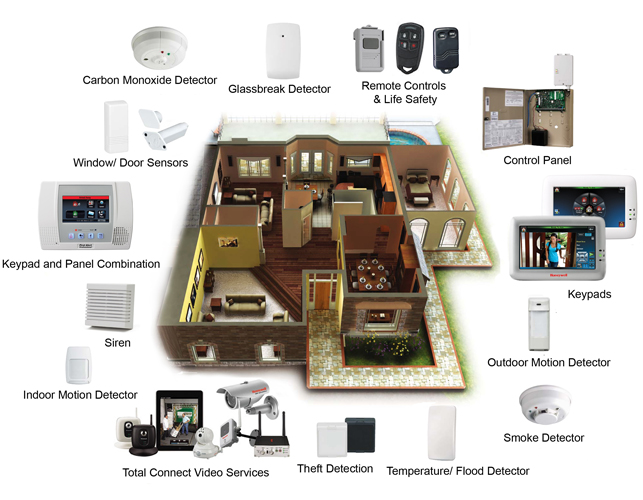
\includegraphics[width=0.9\textwidth]{images/Chapter_02/security.jpg}
	\caption{Example of a smart home with security-oriented devices}
	\label{fig:security-in-smarthome}
\end{figure}

\bigskip
There is not an exact point where we can set the beginning of the domotics as a real concept, but during the last century
there has been some remarkable efforts, and even before. In 1898, Nikola Tesla created a wireless control for a toy boat, 
the first of its kind \cite{betanewsHistory}. That marks the beginning of wireless technologies, one of the fundamental
parts of Home Automation. 

\bigskip
In 1975, after lots of appearances of the idea of home automation in films, the first general purpose home automation
technology, called X10, was developed. X10 defines a protocol for communication between electrical devices, which uses power
line wiring for signaling and control, where the signals involve brief radio frequency bursts representing digital information.
Therefore, it also defines a wireless radio based protocol. Surprisingly, the X10 technology is still widely used and available,
with millions of units in use worldwide.

\bigskip
However, it was not until 1984 that the word Smart Home appeared, invented by the \textit{American Association of House
Builders}. After that, different inventions rapidly followed one another, with devices such as\\ \textit{The Clapper} (which 
was operated through sound, like a clap or a bark) and interest from the biggest technological companies, like Microsoft.

\begin{figure}
	\centering
	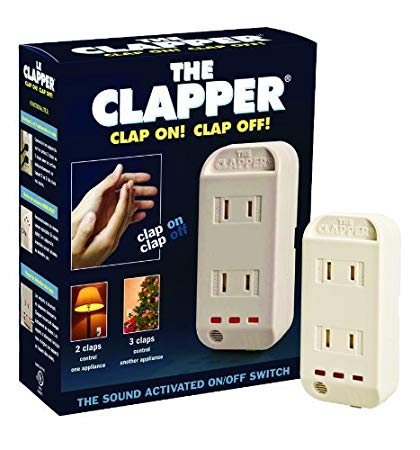
\includegraphics[width=0.5\textwidth]{images/Chapter_02/the-clapper.jpg}
	\caption{The Clapper, a sound-activated switch}
	\label{fig:the-clapper}
\end{figure}

\bigskip
Home Automation has not stopped gaining ground on our homes and now it is experiencing one of the best moments
in its lifetime, with the unstoppable growth of the Internet of Things (IoT) and the simultaneous development of Artificial 
Intelligence for the general public, with the biggest companies, like Google and Apple, investing millions of dollars on it.
Devices like Amazon Echo and Google Home, or assistants like Siri, Cortana, Google Assistant and Amazon Alexa are a 
good representative of this trend. I will talk in depth about them in the following sections.

\bigskip
We have always imagined that Smart Homes would bring us a whole world of benefits. And that is partly true, but
they have ended up offering benefits that no one could imagine some decades before, when matters such as energy
savings were not as important as today. These benefits are responsible for their increasing popularity, and they can be 
summarized in the following points:

\begin{itemize}
	\item \textbf{Control anywhere:} Smart Homes can be completely controlled anywhere in the world from smart phones or
	other devices with Internet connection, so we can know the status of our devices at any time. That would allow us, for
	example, to stop worrying when staging out of home thinking if we have left the air conditioning on.
	\item \textbf{Safety:} there are tons of security systems ready to work on Smart Houses. They are capable of monitoring
	the people going in and out of home and send alerts to the owners if necessary. Like many other devices, there are also
	smart locks for the door and cameras that we can control from our smart device.
	\item \textbf{Accessibility:} Smart Homes can increase a lot the quality of life of elderly or disabled people, as they can be
	managed via voice commands, making the interaction much easier to people which is not experienced with computers and
	improving their independence.
	\item \textbf{Energy efficiency:} one of the main goals of Home Automation is to work with the least amount of energy 
	needed, and a big part of the research in this field is going in this direction. There are induction cook-top stoves that can be 
	powered on only if there is anything placed over them (and even get the perfect cooking, powering off themselves)\cite{directenergyAdvantages}
	or heating systems that power on and off depending on the weather and inner conditions of the home, or even a faucet 
	technology that can maximize shower water usage by shaping the individual droplets of water, so the experience feels 
	almost the same but with less water usage. 
	\item \textbf{Money saving:} the last point leads to another benefit: saving money. Smart Homes can use less energy and 
	water, making a big difference in how much we pay at the end of the month. Reports show that the savings on the energy bill 
	for this reason range from 10\% to 30\%.\cite{directenergyAdvantages}
	\item \textbf{Comfort:} Smart Houses can also help save time. Today, when everyone is trying to make the most of their free
	time, this technology is capable of doing housework, so that people can spend their time on things they enjoy most, or simply 
	gain time  to spend with their families.
\end{itemize}

\bigskip
This range of benefits has made possible to see home automation systems in many homes, but also in offices. Now, almost 
every new house that is built is prepared for domotics, including Internet access points in every room, a big amount of plugs, 
and a lot of space to extend its capabilities in a future. Indeed, the global home automation and security control market is 
expected to reach 12.81 billion dollars by 2020.\cite{reutersResearchMarkets} The following charts is a perfect example of how 
rapidly is growing the Smart Home sector and how powerful it is at this moment, showing the data for the most important Smart
Home market at this moment: the United States.

\begin{figure}
	\centering
	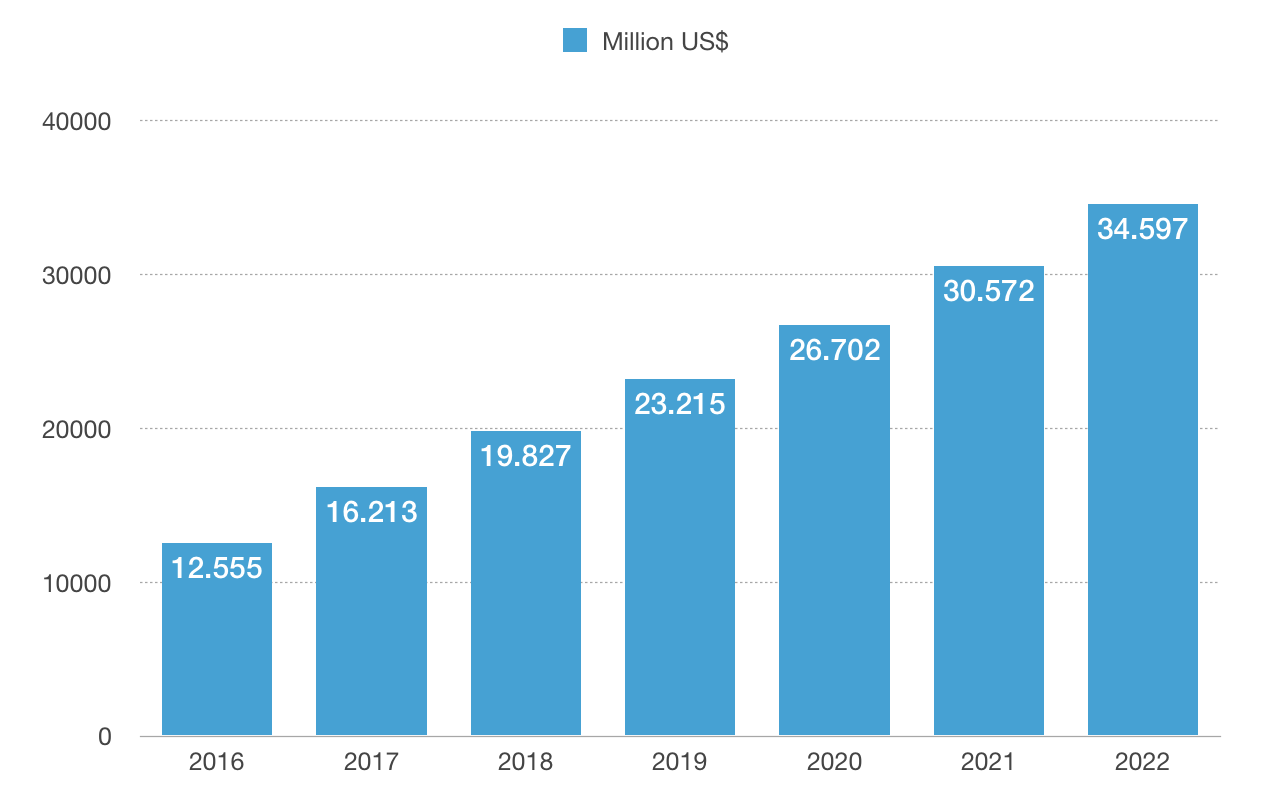
\includegraphics[width=0.9\textwidth]{images/Chapter_02/sh-market-revenue.png}
	\caption{The Smart Home Market revenue from 2016 to 2022 in the US\cite{statistaSmartHomeUS}}
	\label{fig:sh-market-revenue}
\end{figure}

\bigskip
Predictions are not bad either: they show that this trend will continue in the coming years, reaching 34.5 million of the 
US dollars, and this is just in the United States, although there will be similar situations in the rest of the world.

\section{Home Automation System Design}
After a look at the definition and history of Home Automation and its benefits, I am going to explain how these systems are 
usually organized. There is more than one valid way, and it will always depend on the requirements and conditions of the user,
the home environment and of course the capabilities of its components. The figure \ref{fig:sh-basic-structure} is a good 
example of a basic organization for Home Automation\cite{embeddedHASystemDesign}. This organization has a name, indeed:
centralized architecture.

\begin{figure}
	\centering
	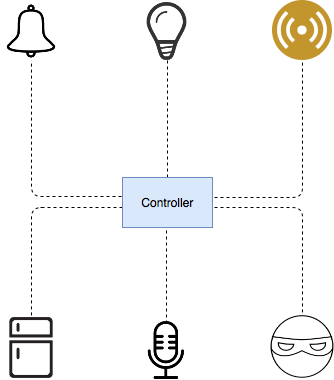
\includegraphics[width=0.55\textwidth]{images/Chapter_02/basic-sh-structure.png}
	\caption{Centralized Smart Home structure}
	\label{fig:sh-basic-structure}
\end{figure}

\subsection{Centralized Architecture}
In a centralized Smart Home Environment architecture, the Control System, which is realized by means of a computer
system, is in charge of acquiring data from sensors, providing a user interface, and executing the control algorithms and 
sending instructions to actuators.\cite{badica13} In the example in the figure \ref{fig:sh-basic-structure}, the sensor (in gold) 
can represent a smoke detector that can trigger the alarm (the actuator) to alert the householders.

\bigskip
The controller is often called Home Gateway, and in this case it is the central computer. It is also responsible of making 
accessible the system via Internet, as well as providing services to the home residents. An option to increase its performance 
while maintaining the same architecture is to limit the functionalities of the Home Gateway to data acquisition, software 
interfacing with domotic devices and basic processing, and to delegate to more powerful servers outside home the most
part of the processing.

\bigskip
This is the most popular architecture in home automation, partly because product manufacturers tend to centralize communications
between their intelligent devices in a hub or gateway of the same brand, which users need to install to operate the rest of the devices.

\subsection{Distributed Architecture}
In a distributed Smart Home Environment architecture, the Control System software is conceptualized and implemented as a 
distributed computing system, that is, a series of intercommunicating computers working together to achieve an end, which in this 
case is running a Smart Home system.

\bigskip
The distributed architecture benefits from the computational resources of smart devices to integrate software components into the 
nodes of the Home Automation network, which produces a big increase in performance and modularity. However, the cost of 
this architecture is significantly higher compared to the centralized architecture, and therefore it is hard to achieve a big degree of
granularity. For this reason, this architecture is often applied conceptually, while still physically centralized into the Home Gateway.



